\section{Fleet performance, cost and outlook}\label{sec:fleet}
\sectionstate{partial}{\texttt{mx\_june\_wft/FLEET\_DIGEST.md}; R10 (cost table)}
\intent{All five chambers: $\sigma_\theta$ = \requote{1.15--2.51\textdegree} with waveforms, better than hits on every plane
(\requote{$\times$1.03--2.2}, halved on det3). CPU cost per plane and tier. Outlook: VMM emulation, in-situ calibration at n\_TOF, two-track fits.}
\analysis{R10}{cost table}
\analysis{C3}{n\_TOF tripwires: chamber C non-linearity on its own bundle}
\begin{figure}[t]
  \centering
  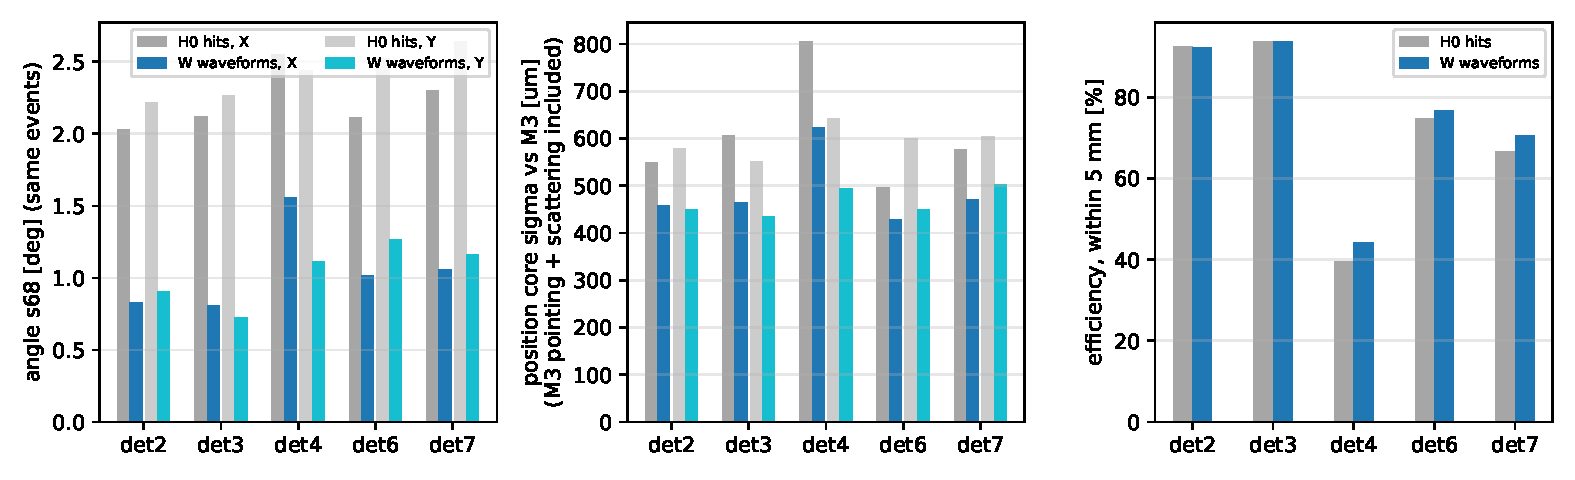
\includegraphics[width=0.9\linewidth]{fleet}
  \caption{\tbw{Fleet performance, hits against waveforms.}}
  \label{fig:fleet}
\end{figure}

\subsection{A known angle in the beam}\label{sec:knownangle}
\sectionstate{open}{R7; \texttt{sps\_beam\_test\_26/analysis/angled\_kernel} (geometry)}
\intent{A reference-free test: det4 rotated by 25.4\textdegree{} (yaw measured from the run-57 alignment; the configuration value was 25.64\textdegree) in the SPS beam. Hits and waveforms against the stage angle,
independent of the M3 telescope.}
\analysis{R7}{known-angle reconstruction, hits vs waveforms}
\begin{figure}[t]
  \centering
  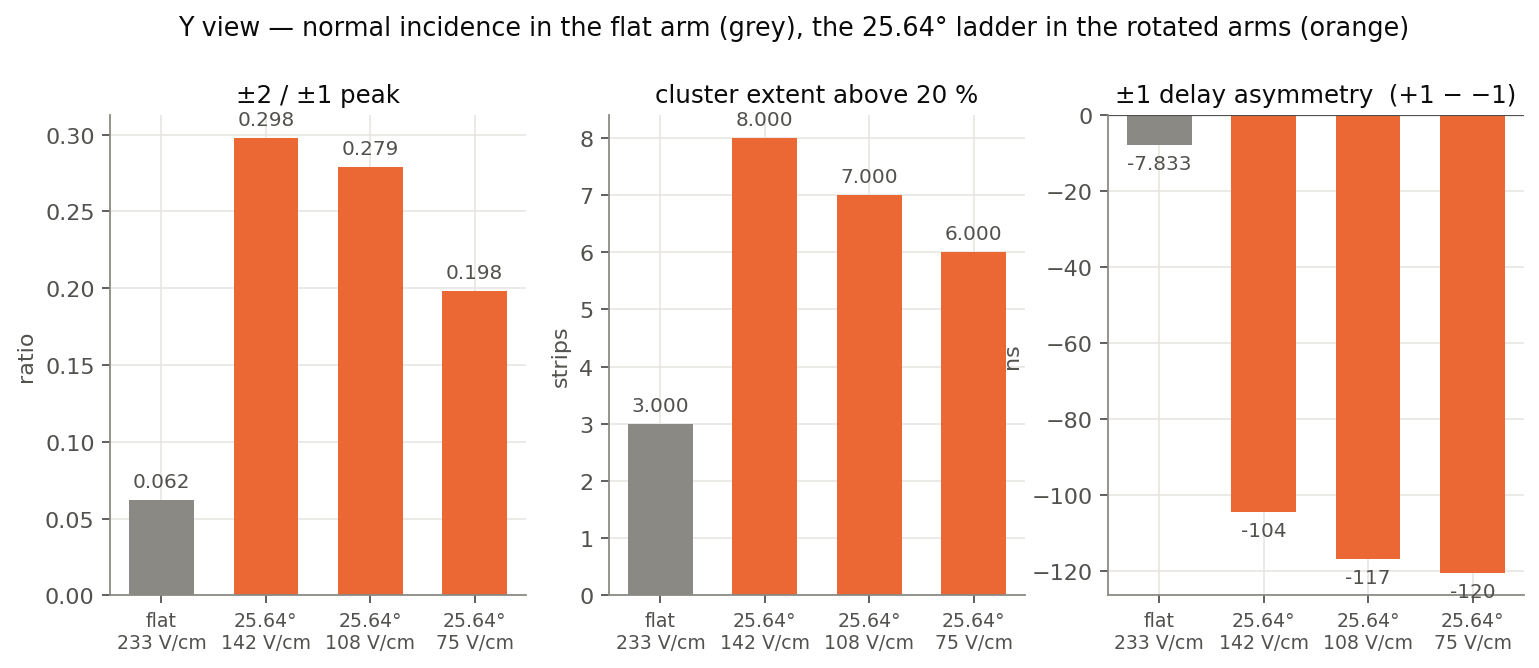
\includegraphics[width=0.6\linewidth]{known_angle_geometry}
  \caption{\tbw{det4 rotated in the beam.}}
  \label{fig:known_angle_geometry}
\end{figure}
\begin{figure}[t]
  \centering
  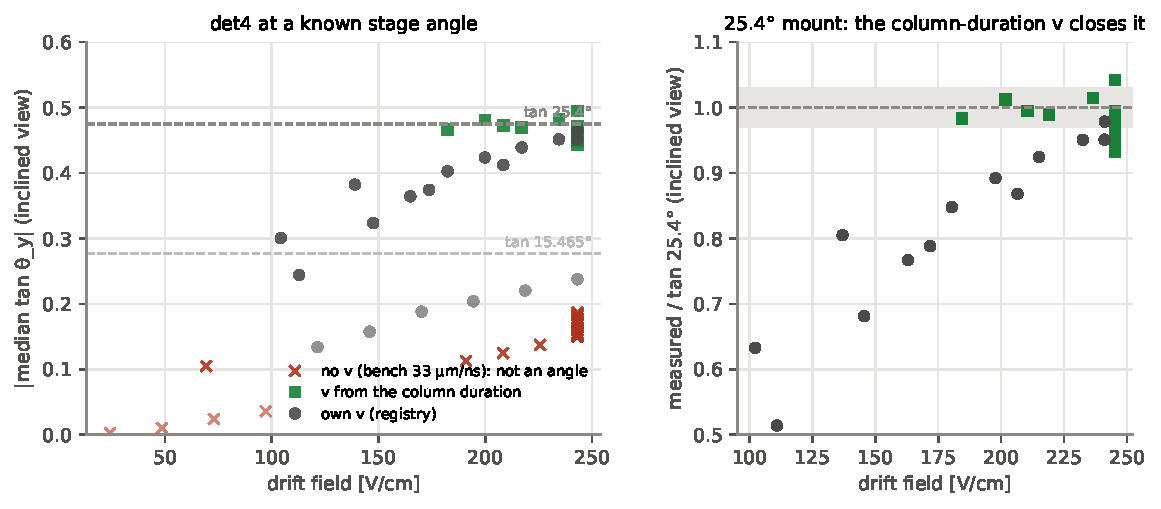
\includegraphics[width=0.7\linewidth]{known_angle}
  \caption{\tbw{Reconstructed angle against the stage angle.}}
  \label{fig:known_angle}
\end{figure}
